% =============================================================================
%  USER MANUAL — DC MOTOR CONTROL LABORATORY EQUIPMENT
%  Department of Systems Engineering and Automation (ISA)
%  Universidad de Sevilla
%  Contact: ialvarado@us.es
% =============================================================================
\documentclass[11pt,a4paper]{article}

% ── Encoding and language ────────────────────────────────────────────────────
\usepackage[utf8]{inputenc}
\usepackage[T1]{fontenc}
\usepackage[english]{babel}

% ── Typography ───────────────────────────────────────────────────────────────
\usepackage{lmodern}
\usepackage{microtype}

% ── Margins ──────────────────────────────────────────────────────────────────
\usepackage[top=2.5cm,bottom=2.5cm,left=2.5cm,right=2.5cm]{geometry}

% ── Graphics and colour ──────────────────────────────────────────────────────
\usepackage{graphicx}
\usepackage[table,xcdraw]{xcolor}
\usepackage{tikz}
\usetikzlibrary{shapes.geometric,arrows.meta,positioning,fit,backgrounds,calc}

% ── Tables ───────────────────────────────────────────────────────────────────
\usepackage{booktabs}
\usepackage{array}
\usepackage{tabularx}
\usepackage{multirow}
\usepackage{longtable}

% ── Source code ──────────────────────────────────────────────────────────────
\usepackage{float}
\usepackage{caption}
\usepackage{listings}
\usepackage{courier}

% ── Notice boxes ─────────────────────────────────────────────────────────────
\usepackage{tcolorbox}
\tcbuselibrary{skins,breakable}

% ── Icons / symbols ──────────────────────────────────────────────────────────
\usepackage{pifont}
\usepackage{amssymb}
% fontawesome5 substitutes
\newcommand{\faInfoCircle}{$\blacksquare$}
\newcommand{\faExclamationTriangle}{$\triangle$}
\newcommand{\faCheckCircle}{\ding{52}}
\newcommand{\faTimesCircle}{\ding{56}}
\newcommand{\faUpload}{$\uparrow$}
\newcommand{\faPlay}{$\blacktriangleright$}

% ── Hyperlinks ───────────────────────────────────────────────────────────────
\usepackage[colorlinks=true,linkcolor=isablue,urlcolor=isablue,citecolor=isablue]{hyperref}

% ── Headers and footers ──────────────────────────────────────────────────────
\usepackage{fancyhdr}
\usepackage{lastpage}

% ── Enhanced lists ───────────────────────────────────────────────────────────
\usepackage{enumitem}

% ── Paragraph spacing ────────────────────────────────────────────────────────
\setlength{\parskip}{4pt}
\setlength{\parindent}{0pt}

% =============================================================================
%  ISA COLOURS
% =============================================================================
\definecolor{isablue}{RGB}{0,70,130}
\definecolor{isared}{RGB}{180,30,30}
\definecolor{isagray}{RGB}{240,242,244}
\definecolor{isagreen}{RGB}{0,120,60}
\definecolor{isaorange}{RGB}{200,90,0}
\definecolor{codebg}{RGB}{248,248,248}

% =============================================================================
%  NOTICE BOXES
% =============================================================================
\newtcolorbox{infobox}[1][]{
  colback=isablue!8, colframe=isablue, fonttitle=\bfseries,
  title={\faInfoCircle\quad Note}, #1
}
\newtcolorbox{warnbox}[1][]{
  colback=isaorange!10, colframe=isaorange, fonttitle=\bfseries,
  title={\faExclamationTriangle\quad Warning}, #1
}
\newtcolorbox{successbox}[1][]{
  colback=isagreen!8, colframe=isagreen, fonttitle=\bfseries,
  title={\faCheckCircle\quad Success}, #1
}
\newtcolorbox{errorbox}[1][]{
  colback=isared!8, colframe=isared, fonttitle=\bfseries,
  title={\faTimesCircle\quad Common issue}, #1
}

% =============================================================================
%  CODE STYLE
% =============================================================================
\lstset{
  basicstyle=\ttfamily\small,
  backgroundcolor=\color{codebg},
  frame=single,
  rulecolor=\color{gray!40},
  breaklines=true,
  columns=fullflexible,
  keepspaces=true,
  showstringspaces=false,
  numbers=none,
}
\lstdefinestyle{matlab}{language=Matlab, keywordstyle=\color{isablue}\bfseries,
  commentstyle=\color{gray}\itshape, stringstyle=\color{isared}}
\lstdefinestyle{bash}{language=bash, keywordstyle=\color{isagreen}\bfseries,
  commentstyle=\color{gray}\itshape}

% =============================================================================
%  HEADER / FOOTER
% =============================================================================
\pagestyle{fancy}
\fancyhf{}
\fancyhead[L]{\textcolor{isablue}{\small\textbf{User Manual — DC Motor Control Equipment}}}
\fancyhead[R]{\textcolor{isablue}{\small ISA · Universidad de Sevilla}}
\fancyfoot[C]{\textcolor{gray}{\small Page \thepage\ of \pageref{LastPage}}}
\renewcommand{\headrulewidth}{0.4pt}
\renewcommand{\footrulewidth}{0pt}
\renewcommand{\headrule}{\color{isablue}\hrule width\headwidth height\headrulewidth}

% =============================================================================
%  TITLE
% =============================================================================
\title{%
  \vspace{-1cm}
  {\color{isablue}\rule{\linewidth}{2pt}}\\[0.5em]
  {\Huge\bfseries\color{isablue} User Manual}\\[0.3em]
  {\Large DC Motor Control Laboratory Equipment}\\[0.3em]
  {\color{isablue}\rule{\linewidth}{0.5pt}}\\[0.6em]
  \includegraphics[width=0.72\linewidth]{equipo_render.png}\\[0.6em]
  {\color{isablue}\rule{\linewidth}{0.5pt}}\\[0.3em]
  {\normalsize Department of Systems Engineering and Automation (ISA)\\
   Universidad de Sevilla \quad·\quad \href{mailto:ialvarado@us.es}{ialvarado@us.es}}
}
\date{\today}
\author{}

% =============================================================================
\begin{document}
% =============================================================================

\maketitle
\thispagestyle{fancy}

% ── Quick summary ─────────────────────────────────────────────────────────
\begin{tcolorbox}[colback=isablue!5,colframe=isablue,fontupper=\small]
\textbf{What this equipment does:} a Maxon DC motor with a 14-bit magnetic encoder,
controlled in closed loop from MATLAB/Simulink via an Arduino.
The control loop \emph{runs entirely on the PC}: the Arduino only reads the encoder
and applies the PWM commanded by MATLAB every \textbf{10\,ms} (100\,Hz).
Communication is via USB/serial at 115\,200\,baud.

\medskip
\textbf{What the instructor needs:} connect the USB cable, select the serial port
in Simulink, and start the experiment. Everything else is automatic.
\end{tcolorbox}

\tableofcontents
\newpage

% =============================================================================
\section{Equipment Description}
% =============================================================================

\subsection{Main Components}

\begin{center}
\begin{tabular}{llp{7.5cm}}
\toprule
\textbf{Component} & \textbf{Model} & \textbf{Function} \\
\midrule
Motor      & Maxon A-max 22 & Precision DC motor with GP\,22\,B planetary gearbox \\
Encoder    & ams AS5047P    & 14-bit magnetic encoder (16\,384 steps/rev), load-side mounted \\
Driver     & TB6612FNG      & Dual motor driver integrated on the shield PCB \\
MCU        & Arduino UNO    & Reads encoder, applies PWM, communicates with MATLAB via USB \\
Shield PCB & ISA custom     & Stacks directly on the Arduino; integrates driver + encoder connector \\
\bottomrule
\end{tabular}
\end{center}

\subsection{Connection Diagram}

\begin{center}
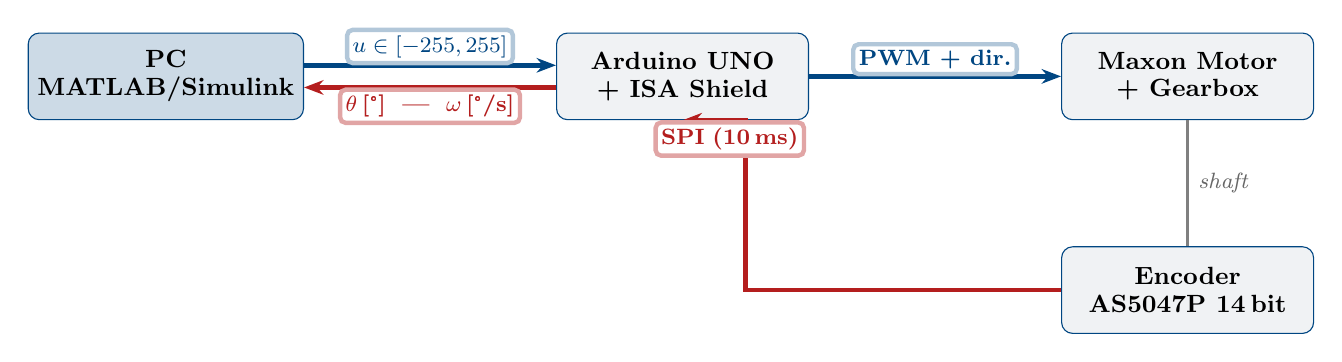
\begin{tikzpicture}[
  block/.style={draw,rounded corners,fill=isagray,minimum width=3.2cm,minimum height=1.1cm,
                align=center,font=\small\bfseries},
  arrow/.style={-{Stealth[length=7pt]},line width=1.6pt,isablue},
  arrowback/.style={-{Stealth[length=7pt]},line width=1.6pt,isared},
  lbl/.style={font=\footnotesize\bfseries, fill=white, draw=isablue!30,
              rounded corners=2pt, inner sep=2pt, text=isablue}
]
  \node[block,fill=isablue!20,draw=isablue] (pc)  {PC\\[-1pt]{\small MATLAB/Simulink}};
  \node[block,fill=isagray,draw=isablue, right=3.2cm of pc]  (ard) {Arduino UNO\\[-1pt]{\small + ISA Shield}};
  \node[block,fill=isagray,draw=isablue, right=3.2cm of ard] (mot) {Maxon Motor\\[-1pt]{\small + Gearbox}};
  \node[block,fill=isagray,draw=isablue, below=1.6cm of mot] (enc) {Encoder\\[-1pt]{\small AS5047P 14\,bit}};

  % PC → Arduino  (control signal)
  \draw[arrow] ([yshift=4pt]pc.east) --
    node[above, lbl]{$u\in[-255,255]$} ([yshift=4pt]ard.west);

  % Arduino → PC  (position + velocity)
  \draw[arrowback] ([yshift=-4pt]ard.west) --
    node[below, lbl, text=isared, draw=isared!40]{$\theta$\,[°] \;|\; $\omega$\,[°/s]} ([yshift=-4pt]pc.east);

  % Arduino → Motor  (PWM + direction)
  \draw[arrow] (ard.east) --
    node[above, lbl]{PWM + dir.} (mot.west);

  % Motor → Encoder  (mechanical shaft)
  \draw[-,line width=1.2pt,black!50] (mot.south) -- (enc.north)
    node[midway, right, font=\footnotesize\itshape, text=black!60]{shaft};

  % Encoder → Arduino  (SPI)
  \draw[arrowback] (enc.west) -| ([xshift=0.8cm]ard.south) -- (ard.south)
    node[near start, below, lbl, text=isared, draw=isared!40]{SPI\;(10\,ms)};

\end{tikzpicture}
\end{center}

\smallskip
{\footnotesize\textcolor{isablue}{$\longrightarrow$} Control signal \quad
 \textcolor{isared}{$\longrightarrow$} System measurements \quad
 \textcolor{black!50}{---} Mechanical coupling}

\begin{infobox}
The complete control loop runs in MATLAB. The Arduino acts as a
\textbf{real-time hardware interface}: it sets the experiment cadence via
Timer2 interrupts every \textbf{10\,ms} (100\,Hz), reads the encoder over SPI,
computes the numerical velocity ($\Delta\theta/T_s$), and applies to the driver the
control signal received from MATLAB.

\smallskip
\textbf{Angle accumulation:} the AS5047P encoder outputs the angle in the range
$[0^{\circ}, 360^{\circ})$ per revolution. The firmware counts complete revolutions and
accumulates the angle, so the output is an unbounded angle $\in(-\infty,+\infty)$
that grows (or decreases) continuously without jumps or resets — just like an
incremental encoder.

\smallskip
\textbf{Luenberger observer} (disabled by default): estimates filtered position and
velocity instead of the raw numerical derivative. Enable it by uncommenting four
lines at the end of the transmit block in \texttt{main.ino}.
\end{infobox}

\subsection{System Parameters}

\begin{center}
\begin{tabular}{lll}
\toprule
\textbf{Parameter} & \textbf{Value} & \textbf{Notes} \\
\midrule
Sampling period $T_s$      & 10\,ms (100\,Hz) & Fixed in Arduino firmware \\
Communication speed        & 115\,200\,baud   & USB/serial \\
Control signal range       & $u \in [-255,\,255]$ & Maps to $\pm V_{\mathrm{supply}}$ (see note) \\
Encoder resolution         & $\approx 0.022^{\circ}$/step & 16\,384 steps/rev \\
Approximate model          & $G(s)=K/(\tau s+1)$ & $K$ and $\tau$ depend on $V_{\mathrm{supply}}$ \\
\bottomrule
\end{tabular}
\end{center}

\begin{warnbox}[title={\faExclamationTriangle\quad Supply Voltage}]
The signal $u \in [-255,\,255]$ maps to $\pm V_{\mathrm{supply}}$, which depends on
how the equipment is powered:
\begin{itemize}[noitemsep,leftmargin=*]
  \item \textbf{External supply (recommended):} max.\ \textbf{9\,V}; in practice
        \textbf{8.4\,V} is recommended to avoid excessive motor heating.
        $u = 255 \Rightarrow 8.4$\,V.
  \item \textbf{USB only (no external supply):} the motor runs at $\approx\pm5$\,V.
        Reduced speed range, but fully functional for initial tests and sessions
        without a bench power supply.
\end{itemize}
The model $G(s)=K/(\tau s+1)$ must be identified experimentally for each
supply voltage used.
\end{warnbox}

% =============================================================================
\section{Initial Setup (one-time only)}
% =============================================================================

This section is only needed the \textbf{first time} the equipment is configured,
or if the Arduino is replaced. It does not need to be repeated each lab session.

\subsection{Install Arduino Libraries}

\begin{enumerate}[leftmargin=*]
  \item Open \textbf{Arduino IDE 2.x}.
  \item Go to \texttt{Tools → Library Manager}.
  \item Search for and install \texttt{AS5047P} (author: Marginally Clever Robots).
  \item Search for and install \texttt{MsTimer2} (author: Javier Valencia).
\end{enumerate}

\begin{infobox}
These libraries only need to be installed once on the lab PC.
If a different computer is used, repeat this step.
\end{infobox}

\subsection{Upload Firmware to the Arduino}

\begin{enumerate}[leftmargin=*]
  \item Connect the Arduino to the PC via USB.
  \item Open the file \texttt{firmware/arduino/main/main.ino} from the repository.
  \item Select the correct board: \texttt{Tools → Board → Arduino UNO}.
  \item Select the port: \texttt{Tools → Port → COMx} (Windows) or
        \texttt{/dev/tty.usbmodem…} (Mac/Linux).
  \item Click the \faUpload\ \textbf{Upload} button (or press \texttt{Ctrl+U}).
  \item Wait for the message \emph{``Upload successful''} to appear.
\end{enumerate}

\begin{successbox}
To verify the firmware is running: open the \textbf{Serial Monitor} in the IDE
(\texttt{Ctrl+Shift+M}) and set it to \texttt{115200 baud}.
You will see \textbf{garbled characters or meaningless symbols} scrolling at high
speed — this is completely normal. The data travels binary-encoded, not as
readable text, so the Serial Monitor displays it as gibberish.
The important thing is that \emph{something appears}: if the screen stays blank,
check the encoder wiring.
\end{successbox}

\begin{warnbox}
The firmware is already loaded on the lab equipment. Only re-upload it if the
Arduino is replaced or the firmware is updated.
\end{warnbox}

\subsection{Check Shield Wiring}

The shield PCB stacks directly on the Arduino (no cables needed).
Verify that:

\begin{itemize}[leftmargin=*]
  \item The shield is fully seated on the Arduino (all pins engaged).
  \item The motor cable is connected to the driver terminals.
  \item The encoder cable (7-pin JST connector) is connected to the shield.
  \item The power supply is connected to the Arduino's power jack
        (recommended: \textbf{8.4\,V}; max.\ 9\,V). Without an external supply,
        the equipment runs on USB alone at $\approx5$\,V.
\end{itemize}

% =============================================================================
\section{Usage in Each Lab Session}
% =============================================================================

This is the standard procedure at the start of each session. With the equipment
already configured, it takes less than two minutes.

\subsection{Step 1 — Connect the Hardware}

\begin{enumerate}[leftmargin=*]
  \item Connect the Arduino USB cable to the PC.
  \item \textbf{Optional:} connect the power supply to the Arduino's barrel connector
        (recommended \textbf{8.4\,V}, max.\ 9\,V). Without an external supply,
        the equipment works on USB alone ($\approx5$\,V) with a reduced speed range.
\end{enumerate}

\begin{figure}[H]
  \centering
  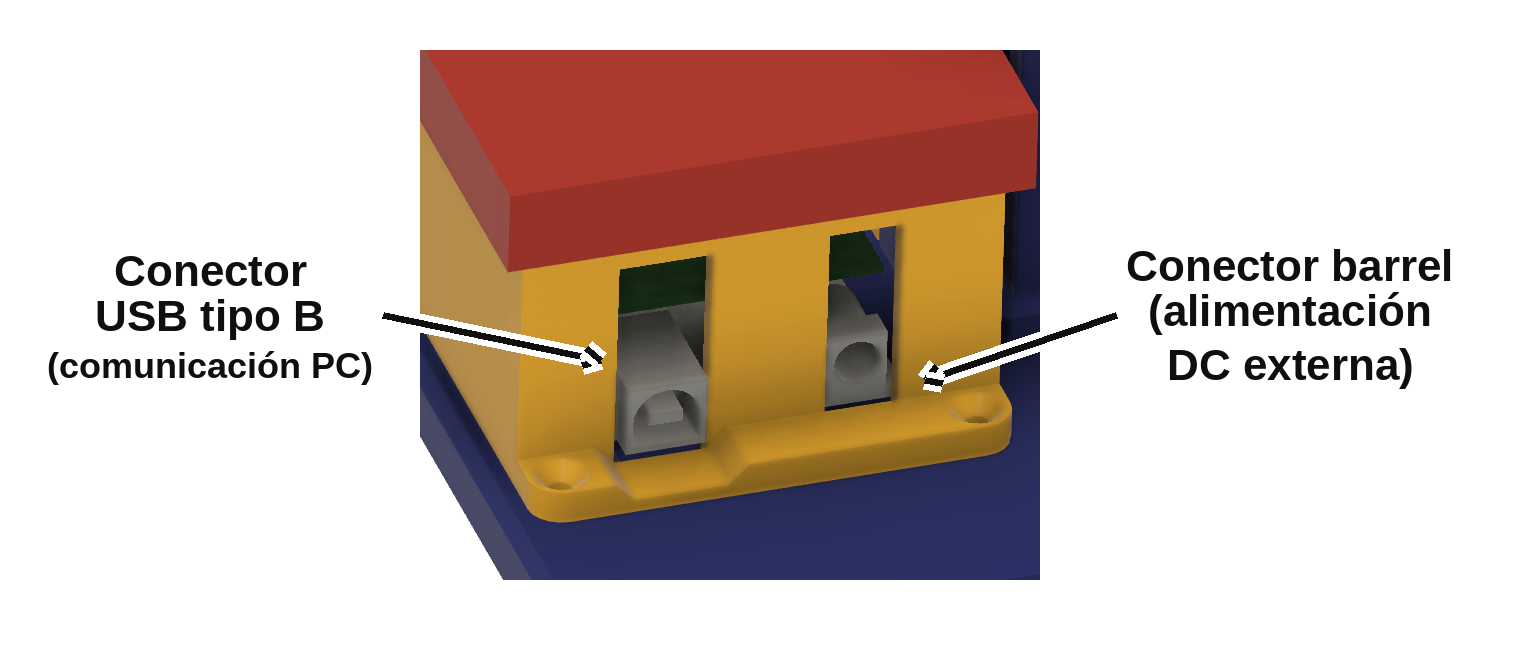
\includegraphics[width=0.68\linewidth]{barrel_connector}
  \caption*{\footnotesize\textit{Front panel detail. Left: USB type-B connector
  (PC communication). Right: \textbf{barrel connector} (external DC power input,
  8.4\,V recommended).}}
\end{figure}

\begin{enumerate}[leftmargin=*, start=3]
  \item The Arduino LED should turn on. \faCheckCircle
\end{enumerate}

\begin{warnbox}
Always connect the USB first, then the external power supply.
When disconnecting, reverse the order: power supply first, then USB.
\end{warnbox}

\subsection{Step 2 — Select the Serial Port in Simulink}

The port is configured directly inside the Simulink model — no additional MATLAB
commands are needed.

\begin{enumerate}[leftmargin=*]
  \item Open the model \texttt{software/matlab/MotorCC\_V3.slx}.
  \item \textbf{Double-click} the central block \textbf{``Motor CC''}.
        A parameter window will open showing a drop-down list of the serial ports
        currently available on the PC.
  \item Select the port that corresponds to the Arduino and click \textbf{OK}.
\end{enumerate}

\begin{infobox}[title={\faInfoCircle\quad Which port is the Arduino?}]
If it is not obvious which port belongs to the Arduino:
\begin{enumerate}[noitemsep]
  \item \textbf{Disconnect} the Arduino USB cable.
  \item Double-click the \textbf{``Motor CC''} block and note the ports in the list.
  \item \textbf{Reconnect} the Arduino USB cable.
  \item Double-click the block again: the new port that now appears is the Arduino.
        Select it and click OK.
\end{enumerate}
\end{infobox}

\subsection{Step 3 — Launch the Experiment from Simulink}

\begin{enumerate}[leftmargin=*]
  \item With the port already selected in the \textbf{``Motor CC''} block (Step 2),
        press the \textbf{Run} button (\faPlay) in the Simulink toolbar.
  \item The model connects automatically to the Arduino and starts the control loop
        at 100\,Hz.
  \item To stop the experiment, press the \textbf{Stop} button.
\end{enumerate}

\begin{warnbox}[title={\faExclamationTriangle\quad Stop the simulation only when the motor is at rest}]
Stopping the simulation (pressing \textbf{Stop}) \emph{while the motor is running}
can be hazardous: when communication is lost, the driver holds the
\textbf{last PWM value} it received indefinitely, and the motor keeps spinning
without control.
Always wait until the motor is \textbf{stopped} (control signal $u = 0$) before
pressing Stop, or bring $u$ to zero from Simulink before stopping.
\end{warnbox}

\begin{successbox}
If everything is working, the Simulink scope will show the angular position (in
degrees) and the applied control signal in real time. The motor will respond to
the configured reference.
\end{successbox}

\subsection{Step 4 — Save Experiment Data}

The model \texttt{MotorCC\_V3.slx} does not include any data-saving blocks: each
student is expected to add the necessary blocks (\emph{To Workspace},
\emph{To File}, \emph{Scope} with auto-save, etc.) to their own model, following
the instructions for each lab assignment.

\begin{infobox}
The variables available each Simulink cycle are: angular position (°),
angular velocity (°/s), and control signal $u \in [-255,255]$.
Refer to each lab guide for the exact blocks to add and the variable names
to use for export.
\end{infobox}

% =============================================================================
\section{Quick Reference}
% =============================================================================

\subsection{Serial Communication Protocol}

\begin{center}
\renewcommand{\arraystretch}{1.25}
\begin{tabularx}{\linewidth}{@{}lX@{}}
\toprule
\textbf{Direction} & \textbf{Binary format and meaning} \\
\midrule
Arduino → MATLAB &
  \texttt{\small 'V' | float(4\,B) | float(4\,B) | float(4\,B) | '\textbackslash n'} \\
  & \quad\textit{angle [°] · velocity [°/s] · applied PWM} \\[4pt]
MATLAB → Arduino &
  \texttt{\small 'A' | int16(2\,B) | '\textbackslash n'} \\
  & \quad\textit{control signal $u \in [-255,255]$} \\
\bottomrule
\end{tabularx}
\end{center}

Transmission rate: \textbf{100\,Hz} ($T_s = 10$\,ms). Binary format (little-endian).

\subsection{Arduino / Shield Pin Assignments}

\begin{center}
\begin{tabular}{lll}
\toprule
\textbf{Arduino Pin} & \textbf{Signal} & \textbf{Description} \\
\midrule
4  & CS (SPI)  & Chip Select — AS5047P encoder \\
11 & MOSI      & SPI MOSI \\
12 & MISO      & SPI MISO \\
13 & CLK       & SPI Clock \\
9  & EnA (PWM) & Enable / PWM — driver channel A \\
7  & Ain1      & Motor direction (bit 1) \\
8  & Ain2      & Motor direction (bit 2) \\
\bottomrule
\end{tabular}
\end{center}

\subsection{Control Signal to Average Motor Voltage}

The TB6612FNG driver switches the supply voltage via PWM.
The \textbf{average voltage} applied to the motor is proportional to the duty cycle:

\[
  \overline{V}_{\mathrm{motor}} = \frac{u}{255} \cdot V_{\mathrm{supply}}
\]

where $V_{\mathrm{supply}}$ is the driver supply voltage (\textbf{8.4\,V} recommended
with an external supply; $\approx$\textbf{5\,V} with USB only).

\smallskip
Examples with $V_{\mathrm{supply}} = 8.4$\,V:
$u = 255 \Rightarrow 8.4$\,V,\; $u = 128 \Rightarrow 4.2$\,V,\; $u = 0 \Rightarrow$ motor stopped.
The sign of $u$ determines the direction of rotation.

% =============================================================================
\section{Troubleshooting}
% =============================================================================

\begin{errorbox}[title={\faTimesCircle\quad Serial port does not appear in MATLAB}]
\begin{itemize}[leftmargin=*,noitemsep]
  \item Check that the USB cable is properly connected.
  \item On Windows: open Device Manager and look for \emph{``Ports (COM \& LPT)''}.
        If a yellow triangle appears, reinstall the CH340 or CP2102 driver.
  \item On Mac: run \lstinline[style=bash]{ls /dev/tty.usb*} in Terminal.
  \item Restart MATLAB after connecting the Arduino.
\end{itemize}
\end{errorbox}

\begin{errorbox}[title={\faTimesCircle\quad Motor does not spin}]
\begin{itemize}[leftmargin=*,noitemsep]
  \item Verify that the power supply is on and correctly connected.
  \item Check that the control signal sent from MATLAB is not 0.
  \item Ensure the motor cables are properly connected to the driver terminals.
  \item If the signal is very small ($|u| < 30$) the motor may not overcome the
        dead-zone (static friction). This is normal; it is addressed in Lab\,02.
\end{itemize}
\end{errorbox}

\begin{errorbox}[title={\faTimesCircle\quad Encoder not responding / position always 0}]
\begin{itemize}[leftmargin=*,noitemsep]
  \item Check the 7-pin JST encoder connector: it must be fully seated.
  \item Open the Arduino IDE Serial Monitor at 115\,200\,baud: if no data appears,
        the encoder is not initialising. The firmware prints an error message in that case.
  \item Verify that the shaft magnet is correctly aligned above the encoder
        (recommended air gap: 0.5\,--\,1.5\,mm).
\end{itemize}
\end{errorbox}

\begin{errorbox}[title={\faTimesCircle\quad Simulink disconnects mid-experiment}]
\begin{itemize}[leftmargin=*,noitemsep]
  \item This usually happens when another programme is using the same serial port
        (e.g.\ the Arduino IDE Serial Monitor).
        \textbf{Close the Serial Monitor before launching Simulink.}
  \item If the problem persists, disconnect and reconnect the USB cable and
        relaunch the model.
\end{itemize}
\end{errorbox}

\begin{errorbox}[title={\faTimesCircle\quad Velocity signal is very noisy}]
\begin{itemize}[leftmargin=*,noitemsep]
  \item This is expected: velocity is obtained as the position difference divided
        by $T_s$, which amplifies quantisation noise from the encoder.
  \item Solution: apply a first-order low-pass filter in MATLAB/Simulink with
        time constant $T_f \approx 0.02$\,--\,$0.05$\,s. Covered in Lab\,01.
\end{itemize}
\end{errorbox}

% =============================================================================
\section{Repository and Resources}
% =============================================================================

\begin{center}
\begin{tabular}{ll}
\toprule
\textbf{Resource} & \textbf{Location} \\
\midrule
Full repository      & \href{https://github.com/DocMuerde/Motor-CC-Control-Lab}{\texttt{github.com/DocMuerde/Motor-CC-Control-Lab}} \\
Arduino firmware     & \texttt{firmware/arduino/main/main.ino} \\
MATLAB scripts       & \texttt{software/matlab/} \\
Simulink model       & \texttt{software/matlab/MotorCC\_V3.slx} \\
Lab guide — Lab\,01  & \texttt{labs/lab01/lab01\_isa.pdf} \\
Lab guide — Lab\,02  & \texttt{labs/lab02/lab02\_isa.pdf} \\
PCB schematics       & \texttt{hardware/pcb/} \\
3D-printed parts     & \texttt{hardware/3d-printing/} \\
\bottomrule
\end{tabular}
\end{center}

\begin{infobox}
To clone the full repository:
\begin{lstlisting}[style=bash]
git clone https://github.com/DocMuerde/Motor-CC-Control-Lab.git
\end{lstlisting}
\end{infobox}

\vfill
{\color{isablue}\rule{\linewidth}{0.5pt}}\\[0.3em]
{\small\color{gray}
Department of Systems Engineering and Automation (ISA) ·
Universidad de Sevilla ·
\href{mailto:ialvarado@us.es}{ialvarado@us.es} ·
\today
}

\end{document}
